
\chapter{Linear Analysis of Numerical Methods}
\label{chp:AnalNumMethod}
The most important property of a numerical method is convergence. Convergence guarantees that as we increase the spatial and temporal resolution of a numerical method, its numerical solution approaches the solution of the partial differential equations. For linear partial differential equations the Lax-equivalence theorem states that a numerical method is convergent if and only if it is stable and consistent \cite{Lax-Richtmyer-1956-267}. Where consistency means that the error introduced by the numerical method at every time step approaches zero as the spatial and temporal resolution is increased. While stability means that the errors from all previous time steps are not amplified by each evolution step.

The convergence of the finite difference methods introduced in Chapter [] has not been shown for the Serre equations and so we investigate it here. The consistency of the finite difference methods follows from our use of well tested approximations and so we instead focus on demonstrating the stability for these methods. In particular we performed a Von Neumann stability \cite{Charney-etal-1950-237} analysis on the finite difference methods applied to the linearised Serre equations.

Another property of the Serre equations is that it possesses a dispersion relation that well approximates the dispersion relation for the Euler equations. For this reason we wish to know the error in the dispersion relation for all the numerical methods we are interested in; the finite difference volume methods and the finite element volume methods. 

The aim of both analyses is to produce a relationship between the primitive variables $h$ and $u$ at the current time level to the primitive variables at the next time level of the form
\begin{equation}
\label{eqn:linearanalaim}
\begin{bmatrix}
h \\u
\end{bmatrix}^{n+1}_j = \matr{E} \begin{bmatrix}
h \\u
\end{bmatrix}^{n}_j
\end{equation}
where $\matr{E}$ is the evolution matrix. The evolution matrix $\matr{E}$ is obtained in the analyses by propagating Fourier modes through the numerical scheme applied to the linearised Serre equations with horizontal beds. We neglect bed terms because variations in the bed have no effect on the dispersion relation. We begin by giving the linearised equations, performing the dispersion relation analysis and then performing the stability analysis.
 
\section{Linearised Serre equations with horizontal bed}
The Serre equations with a horizontal bed \eqref{eqn:FullSerreNonConHorizbed} are linearised by considering waves as small perturbations $\delta\eta$ and $\delta\upsilon$ on a flow with a mean height $H$ and a mean velocity $U$ respectively

\begin{align}
\label{eq:pertubation}
h(x,t) &= H + \delta \eta(x,t) + \mathcal{O}\left(\delta^2 \right), \\
u(x,t) &= U + \delta \upsilon(x,t) + \mathcal{O}\left(\delta^2 \right),
\end{align}
where $\delta \ll 1$. These waves are relatively small so terms of order $\delta^2$ are negligible. We substitute \eqref{eq:pertubation} into the Serre equations and neglect terms of order $\delta^2$ to obtain

\begin{subequations}
	\begin{gather}
		\label{eqn:LinCont}
		\frac{\partial  \left(\delta\eta \right)}{\partial  t} + H\frac{\partial  \left(\delta\upsilon \right)}{\partial  x} + U\frac{\partial  \left(\delta\eta \right)}{\partial  x}  = 0,
	\end{gather}
	\begin{gather}
	\label{eqn:LineMome}
	H\frac{\partial  \left(\delta\upsilon \right)}{\partial  t} + gH\frac{\partial  \left(\delta\eta \right)}{\partial  x} + UH\frac{\partial  \left(\delta\upsilon \right)}{\partial  x} - \frac{H^3}{3}\left(U\frac{\partial^3  \left(\delta\upsilon \right)}{\partial  x^3} + \frac{\partial^3  \left(\delta\upsilon \right)}{\partial  x^2 \partial  t}  \right)  = 0
	\end{gather}
\label{eqn:LinSerre}	
and for $G$
\begin{gather}
	G = UH + U \delta \eta + H \delta \upsilon -\frac{H^3}{3} \frac{\partial^2 \left(\delta\upsilon \right)}{\partial x^2}.
	\label{eqn:LinConSerreG}
\end{gather}	
\end{subequations}

%Phillipine stuff in here%
\section{Dispersion Relation Analysis}
To study the error in the dispersion relation caused by the numerical methods we will follow the work of \cite{Filippini-etal-2016-381}. We will demonstrate this analysis for one example; the second order FDVM. We will then show how the analysis extends to the FEVM and then present all the derived factors for every FDVM and FEVM. We will then compare the dispersion errors of all FDVM and FEVM.

We begin by assuming that $U = 0$, so that there is no mean flow velocity as in \cite{Filippini-etal-2016-381}. This is a reasonable simplification because for most ocean wave applications we are interested in modelling waves on quiescent water.

Equations \eqref{eqn:LinSerre} reduce to

\begin{subequations}
	\label{eqn:LinSerreu0}
	\begin{gather}
	\label{eqn:LinContu0}
	\frac{\partial  \eta}{\partial  t} + H\frac{\partial  \upsilon}{\partial  x} = 0,
	\end{gather}
	\begin{gather}
	\label{eqn:LineMomeu0}
	H\frac{\partial  \upsilon}{\partial  t} + g H \frac{\partial  \eta}{\partial  x} - \frac{H^3}{3}\left(\frac{\partial^3  \upsilon}{\partial  x^3 \partial  t}  \right)  = 0
	\end{gather}	
with
	\begin{gather}
	G = H\upsilon -\frac{H^3}{3} \frac{\partial^2 \upsilon}{\partial x^2}.
	\label{eqn:LinConSerreGu0}
	\end{gather}	
\end{subequations}
Where we have absorbed the $\delta$ factor into the corresponding terms $\eta$ and $\upsilon$ to ease notation. The linearised equations \eqref{eqn:LinSerreu0} can be reformulated 
\begin{subequations}
	\begin{gather}
	\label{eqn:LinContG}
	\frac{\partial  \eta}{\partial  t} + H\frac{\partial  \upsilon}{\partial  x} = 0,
	\end{gather}
	\begin{gather}
	\label{eqn:LineMomeG}
	\frac{\partial  G}{\partial  t} + g H \frac{\partial  \eta}{\partial  x}  = 0.
	\end{gather}
	\label{eqn:LinSerreG}	
\end{subequations}
These will be the equations we will apply our numerical methods to in order to calculate their dispersion relation.

The final assumption of this analysis is that $\eta$ and $\upsilon$ are periodic functions in both space and time. In particular, we assume that these quantities are Fourier modes, which for a general quantity $q$ means
\begin{equation}
q(x,t) = q(0,0) e^{i\left(\omega t + kx\right)}.
\label{eqn:FourierNode}
\end{equation}
This is precisely the assumption made to derive the analytical dispersion relation of the linearised Serre equations. A consequence of these quantities being Fourier modes and our use of uniform temporal and spatial grids is that for any real numbers $m$ and $l$ we have
\begin{equation}
q^{n + m}_{j + l} = q^n_j e^{ i \left(m \omega \Delta t + l k \Delta x\right)}.
\label{eqn:fourierfactor}
\end{equation}




\subsection{Overview of the analysis}
We will now present a brief overview of how this analysis progresses for a single evolution step of the second-order FDVM. The dispersion analysis will extend to the Runge-Kutta steps which use multiple evolution steps to increase the temporal order of accuracy. How multiple evolution steps interact to determine the dispersion relation will be demonstrated in Subsection \ref{subsec:RKstepdisp}.

For the second-order FDVM the evolution step progresses by
\begin{enumerate}
	\item Given the vectors of the cell averages $\overline{\vecn{\eta}}$ and $\overline{\vecn{G}}$ at the current time.
	\item We use the map $\mathcal{M}$ between cell averages and nodal values to calculate the nodal values ${\vecn{\eta}}$ and ${\vecn{G}}$ from the cell average values $\overline{\vecn{\eta}}$ and $\overline{\vecn{G}}$ so that
	\begin{align*}
	&{\vecn{\eta}} = \mathcal{M}\left(\overline{\vecn{\eta}} \right), 
	&{\vecn{G}} = \mathcal{M}\left(\overline{\vecn{G}} \right). 
	\end{align*}
	\item We use the map $\mathcal{G}$ given by the elliptic equation between $G$ and $\upsilon$ to calculate ${\vecn{\upsilon}}$ from ${\vecn{G}}$ and $H$
	\[{\vecn{\upsilon}} = \mathcal{G}\left(H, {\vecn{G}}\right)\]
	\item We reconstruct $\eta$ and $G$ at the cell interface $x^-_{j+1/2}$ and $x^+_{j+1/2}$ from the cell average values using $\mathcal{R}^{-}$ and $\mathcal{R}^{+}$. We reconstruct $\upsilon$ at the cell interface from the nodal values using $\mathcal{R}^{\upsilon}$. So we have
	\begin{align*}
	&\eta^-_{j+1/2} = \mathcal{R}^{-}\left(\bar{\vecn{\eta}}\right),  &G^-_{j+1/2} = \mathcal{R}^{-}\left(\bar{\vecn{G}}\right), \\
	&\eta^+_{j+1/2} = \mathcal{R}^{+}\left(\bar{\vecn{\eta}}\right),  &G^+_{j+1/2} = \mathcal{R}^{+}\left(\bar{\vecn{G}}\right), \\
	&\upsilon_{j+1/2} = \mathcal{R}^{\upsilon}\left({\vecn{\upsilon}}\right).
	\end{align*}
	\item We calculate $F_{j+1/2}$ using $\mathcal{F}$
	\[F_{j+1/2} =\mathcal{F} \left(\eta^-_{j+1/2}, G^-_{j+1/2},\eta^+_{j+1/2}, G^+_{j+1/2},\upsilon_{j+1/2}  \right). \]
	\item We repeat this process for each cell edge and then apply the update formula \eqref{eqn:evolupdatescheme} to evolve the vectors $\overline{\vecn{\eta}}$ and $\overline{\vecn{G}}$ from the current time level to the next time level.
\end{enumerate}
This analysis uses the fact that $\upsilon$, $\eta$ and $G$ are Fourier modes and so we have relations between our quantities at different grid points \eqref{eqn:fourierfactor}. Together with the fact that these operators are just linear combinations of the quantities at different grid points, to derive factors for the operators $\mathcal{M}$, $\mathcal{G}$, $\mathcal{R}^{-}$, $\mathcal{R}^{+}$ and $\mathcal{R}^{\upsilon}$ that is the same for every time step and grid point.

For example we have in the case of the map between cell averages and nodal values $\mathcal{M}$ that this process for $\eta$ leads to
\[\eta_j = \mathcal{M} \overline{\eta}_j.\]
Where $\mathcal{M}$ does not depend on the particular cell or time level.

These operators are combined to give the matrix $\matr{F}$ that calculates the flux at the current time allowing us to write the update formula \eqref{eqn:evolupdatescheme} as

\begin{equation*}
\begin{bmatrix}
\eta \\ \upsilon
\end{bmatrix}^{n+1}_j = \left(\matr{I}  - \Delta t \matr{F} \right) \begin{bmatrix}
\eta \\ \upsilon
\end{bmatrix}^{n}_j = \matr{E} \begin{bmatrix}
\eta \\ \upsilon
\end{bmatrix}^{n}_j
\end{equation*}
in terms of primitive variables as in \eqref{eqn:linearanalaim} for a single forward Euler step. From this equation the dispersion relation of the method can be calculated for a single forward Euler step. 

\subsection{Nodal Values to Cell Averages $\mathcal{M}$}
For the second-order FDVM we use the fact that for a general quantity $q$ we have that
\begin{equation*}
q_j = \overline{q}_j + \mathcal{O}\left(\Delta x^2\right).
\end{equation*}
%
So to attain second-order accuracy we use
%
\begin{equation}
\label{eqn:Mfactorfourier}
q_j = \overline{q}_j  = \mathcal{M} \overline{q}_j.
\end{equation}
Therefore we have a factor $\mathcal{M}$ representing the map between cell averages and nodal values for our numerical method that is constant for every grid point and time step, as desired.


\subsection{Elliptic Equation}

For the second-order finite difference method the derivative in \eqref{eqn:LinConSerreGu0} is approximated by   
\[ \left(\frac{\partial^2 \upsilon}{\partial x^2}\right)_j = \frac{\upsilon_{j-1} - 2\upsilon_{j} + \upsilon_{j+1}}{\Delta x^2}.\]
Making use of \eqref{eqn:fourierfactor} this becomes
\[ \left(\frac{\partial^2 \upsilon}{\partial x^2}\right)_j = \frac{\upsilon_{j} e^{-ik\Delta x} - 2\upsilon_{j} + \upsilon_{j}e^{ik\Delta x}}{\Delta x^2} = \frac{ 2\cos\left(k\Delta x\right) - 2 }{\Delta x^2} \upsilon_{j}.\]

Substituting this approximation into our elliptic equation \eqref{eqn:LinConSerreGu0} one obtains
\begin{equation}
\label{eqn:Gfactorfourier}
\upsilon_j = \frac{3 \Delta x^2}{3 \Delta x^2 H - H^3 \left(2\cos\left(k\Delta x\right) - 2\right)} G_{j} = \mathcal{G} G_{j}.
\end{equation}

\subsection{Reconstruction}
We reconstruct $\eta$ and $G$ at $x^-_{j+1/2}$ and $x^+_{j+1/2}$ as we allow these quantities to be discontinuous across the cell interfaces in our finite volume method. However, since we are assuming that these quantities are Fourier modes and therefore smooth we do not need to use non-linear limiters to ensure our scheme is TVD. Therefore our reconstruction scheme for $\eta$ and $G$ written for a general quantity $q$ is

\begin{equation*}
q^-_{j+\frac{1}{2}} = \overline{q}_j + \frac{- \overline{q}_{j - 1} + \overline{q}_{j+ 1} }{4}
\end{equation*}
and
\begin{equation*}
q^+_{j+\frac{1}{2}} = \overline{q}_{j+1} + \frac{- \overline{q}_{j} + \overline{q}_{j+ 2}}{4}.
\end{equation*}

Using \eqref{eqn:fourierfactor} and \eqref{eqn:Mfactorfourier} these equations become

\begin{subequations}
\label{eqn:RpmfactorFDVM}
\begin{multline}
q^-_{j+\frac{1}{2}} =\frac{1}{\mathcal{M}}{q}_j + \frac{- \frac{1}{\mathcal{M}}{q}_{j} e^{-ik\Delta x} + \frac{1}{\mathcal{M}}{q}_{j} e^{ik\Delta x}}{4} \\= \frac{1}{\mathcal{M}}\left(1  + \frac{i\sin\left(k\Delta x\right)}{2} \right)q_j =\mathcal{R}^- q_j
\end{multline}
and
\begin{multline}
q^+_{j+\frac{1}{2}} = \frac{1}{\mathcal{M}}{q}_{j}e^{ik\Delta x} + \frac{- \frac{1}{\mathcal{M}}{q}_{j} + \frac{1}{\mathcal{M}}_2{q}_{j}e^{2ik\Delta x} }{4} \\= \frac{1}{\mathcal{M}}e^{ik\Delta x}\left(1  - \frac{i\sin\left(k\Delta x\right)}{2} \right){q}_{j} = \mathcal{R}^+ q_j.
\end{multline}
\end{subequations}
These are the reconstruction factors for both $\eta$ and $G$.


In our numerical methods the reconstruction of $\upsilon$ is slightly different as we use nodal values and assume $\upsilon$ is continuous across the cell interface; therefore we only reconstruct $\upsilon$ at $x_{j+1/2}$. For the second order finite difference volume method we have
\begin{equation*}
\upsilon_{j + 1/2} = \frac{\upsilon_{j+1} + \upsilon_{j}}{2}.
\end{equation*}

Using \eqref{eqn:fourierfactor} we obtain

\begin{equation}
\label{eqn:2ndreconu}
\upsilon_{j + 1/2} = \frac{e^{ik\Delta x } + 1}{2} \upsilon_{j} = \mathcal{R}^\upsilon \upsilon_{j} .
\end{equation}
 

\subsection{Flux calculation}
To calculate the flux $F_{j+1/2}$ we use Kurganov's method \cite{Kurganov-etal-2001-707} [eqref].
For the linearised Serre equations we have the wave speed bounds \eqref{eqn:WaveVelocitiesBound}, so that
\begin{align}
a^-_{j+ 1/2} =  - \sqrt{g H}& &\text{and}& &a^+_{j+ 1/2} = \sqrt{g H}.
\end{align}
 Substituting these into our average flux approximation [eqref] we obtain $F_{j+\frac{1}{2}}$ for a general quantity $q$
\begin{equation}\label{eqn:HLL_fluxred}
F_{j+\frac{1}{2}} = \dfrac{ f\left(q^-_{j+\frac{1}{2}}\right) + f\left(q^+_{j+\frac{1}{2}}\right)}{ 2}  - \dfrac{ \sqrt{gH}}{ 2} \left [ q^+_{j+\frac{1}{2}} - q^-_{j+\frac{1}{2}} \right ].
\end{equation}

Substituting in $\eta$ for $q$ in \eqref{eqn:HLL_fluxred} we get that the Kurganov approximation to the flux of $\eta$ \eqref{eqn:LinContG} is
\begin{equation}
\label{eqn:HLL_fluxeta}
F^{\eta}_{j+\frac{1}{2}} = \dfrac{ H \upsilon ^-_{j+\frac{1}{2}}+ H \upsilon ^+_{j+\frac{1}{2}}}{ 2}  - \dfrac{ \sqrt{gH}}{ 2} \left [ \eta^+_{j+\frac{1}{2}} - \eta^-_{j+\frac{1}{2}} \right ]
\end{equation}
Substituting the appropriate reconstruction coefficients \eqref{eqn:RpmfactorFDVM} and \eqref{eqn:2ndreconu} into \eqref{eqn:HLL_fluxeta} results in
\begin{equation}
\label{eqn:etafluxapprox}
F^{\eta}_{j+\frac{1}{2}} = H \mathcal{R}^\upsilon \upsilon_{j}   - \dfrac{ \sqrt{gH}}{ 2} \left [  \mathcal{R}^+ -  \mathcal{R}^- \right ] {\eta}_j  = \mathcal{F}^{\eta,\upsilon} \upsilon_{j}   +  \mathcal{F}^{\eta,\eta} {\eta}_j
\end{equation}

Substituting in $G$ for $q$ in \eqref{eqn:HLL_fluxred} we get that the Kurganov approximation to the flux average for $G$ \eqref{eqn:LinContG} is
\begin{equation}
\label{eqn:HLL_fluxG}
F^{G}_{j+\frac{1}{2}} = \dfrac{ gH \eta ^-_{j+\frac{1}{2}}+ gH \eta ^+_{j+\frac{1}{2}}}{ 2}  - \dfrac{ \sqrt{gH}}{ 2} \left [ G^+_{j+\frac{1}{2}} - G^-_{j+\frac{1}{2}} \right ].
\end{equation}
Substituting in the appropriate reconstruction coefficients \eqref{eqn:RpmfactorFDVM} into \eqref{eqn:HLL_fluxG} and making use of \eqref{eqn:Gfactorfourier} we get that
\begin{equation}
\label{eqn:Gfluxapprox}
F^{G}_{j+\frac{1}{2}} = gH \dfrac{\mathcal{R}^- + \mathcal{R}^+ }{ 2} \eta_j + - \dfrac{ \sqrt{gH}}{ 2} \left [  \mathcal{R}^+ -  \mathcal{R}^- \right ] \frac{1}{\mathcal{G}} \upsilon_j =  \mathcal{F}^{G,\eta} \eta_{j}  + \mathcal{F}^{G,\upsilon}\upsilon_j.
\end{equation}

\subsection{Evolution Matrix}

By substituting our flux approximations \eqref{eqn:etafluxapprox} and \eqref{eqn:Gfluxapprox} into our update scheme \eqref{eqn:evolupdatescheme} and making use of \eqref{eqn:Mfactorfourier} our second order finite difference volume method can be written as

\begin{align*}
\eta^{\,n + 1}_{j} &=  \eta^{\,n }_{j} - \mathcal{M} \frac{\Delta t}{\Delta x}  \left[ \left(\mathcal{F}^{\eta,\eta} \eta_{j}  + \mathcal{F}^{\eta,\upsilon} \upsilon_j \right) - \left(\mathcal{F}^{\eta,\eta} \eta_{j-1}  + \mathcal{F}^{\eta,\upsilon} \upsilon_{j-1} \right)  \right], \\
 G^{\,n + 1}_{j} &= G^{\,n }_{j} - \mathcal{M}\frac{\Delta t}{\Delta x}  \left[ \left(  \mathcal{F}^{G,\eta} \eta_{j}  + \mathcal{F}^{G,\upsilon} \upsilon_j \right) - \left(  \mathcal{F}^{G,\eta} \eta_{j-1}  + \mathcal{F}^{G,\upsilon} \upsilon_{j-1} \right) \right].
\end{align*}

	
Furthermore by making use of \eqref{eqn:fourierfactor} and transforming $G$ into $\upsilon$ using $\mathcal{G}$ \eqref{eqn:Gfactorfourier} we obtain
	
\begin{align*}
\eta^{\,n + 1}_{j} &=  \eta^{\,n }_{j} - \mathcal{M} \frac{\Delta t}{\Delta x}  \left[ \left(1 - e^{-ik\Delta x}\right)\left(\mathcal{F}^{\eta,\eta} \eta_{j}  + \mathcal{F}^{\eta,\upsilon} \upsilon_j \right)  \right], \\
\upsilon^{\,n + 1}_{j} &= \upsilon^{\,n }_{j} - {\mathcal{G}}{\mathcal{M}}\frac{\Delta t}{\Delta x}  \left[ \left(1 - e^{-ik\Delta x}\right)\left(  \mathcal{F}^{G,\eta} \eta_{j}  + \mathcal{F}^{G,\upsilon} \upsilon_j \right) \right].
\end{align*}


This can be written in matrix form as

\begin{multline}
\label{eqn:singleEvolveStep}
\begin{bmatrix}
\eta \\ \upsilon
\end{bmatrix}^{n+1}_j = \begin{bmatrix}
\eta \\ \upsilon
\end{bmatrix}^{n}_j - \frac{\left(1 - e^{-ik\Delta x}\right)\mathcal{M} \Delta t}{ \Delta x}\begin{bmatrix}
\mathcal{F}^{\eta,\eta} & \mathcal{F}^{\eta,\upsilon} \\ \mathcal{G}\mathcal{F}^{G,\eta} & \mathcal{G}\mathcal{F}^{G,\upsilon} 
\end{bmatrix}\begin{bmatrix}
\eta \\ \upsilon
\end{bmatrix}^{n}_j \\= \left(\matr{I}  - \Delta t \matr{F} \right) \begin{bmatrix}
\eta \\ \upsilon
\end{bmatrix}^{n}_j
\end{multline}
for a single Euler step as desired.

\subsection{SSP Runge-Kutta Time Stepping}
\label{subsec:RKstepdisp}
Since we have demonstrated this process for a single evolution step the analysis will now proceed to the SSP Runge-Kutta time stepping that allows our schemes to be temporally higher order accurate.

The second order SSP Runge Kutta time stepping proceeds as follows

\begin{subequations}
	\label{eqn:RKstepfull}
	\begin{equation}
	\label{eqn:RKstepfullp1}
	\begin{bmatrix}
	\eta \\ \upsilon
	\end{bmatrix}^{1}_j = \left(\matr{I} - \Delta t\matr{F} \right)\begin{bmatrix}
	\eta \\ \upsilon
	\end{bmatrix}^{n}_j,
	\end{equation}
	
	\begin{equation}
	\label{eqn:RKstepfullp2}
	\begin{bmatrix}
	\eta \\ \upsilon
	\end{bmatrix}^{2}_j = \left(\matr{I} - \Delta t\matr{F} \right)\begin{bmatrix}
	\eta \\ \upsilon
	\end{bmatrix}^{1}_j,
	\end{equation}
		
	\begin{equation}
	\label{eqn:RKstepfullp3}
	\begin{bmatrix}
	\eta \\ \upsilon
	\end{bmatrix}^{n+1}_j = \frac{1}{2} \left(\begin{bmatrix}
	\eta \\ \upsilon
	\end{bmatrix}^{n}_j + \begin{bmatrix}
	\eta \\ \upsilon
	\end{bmatrix}^{2}_j\right) .
	\end{equation}
\end{subequations}


Substituting \eqref{eqn:RKstepfullp1} and \eqref{eqn:RKstepfullp2} into \eqref{eqn:RKstepfullp3} we can write this in terms of the flux matrix $\matr{F}$ and the primitive variables at $t^n$ as
\begin{equation*}
\begin{bmatrix}
\eta \\ \upsilon
\end{bmatrix}^{n+1}_j = \frac{1}{2} \left(\begin{bmatrix}
\eta \\ \upsilon
\end{bmatrix}^{n}_j + \left(\matr{I} - \Delta t\matr{F} \right)^2 \begin{bmatrix}
\eta \\ \upsilon
\end{bmatrix}^{n}_j\right).
\end{equation*}

Expanding $\left(\matr{I} - \Delta t\matr{F} \right)^2$ we get

\begin{equation}
\label{eqn:FullyExpandedF}
\begin{bmatrix}
\eta \\ \upsilon
\end{bmatrix}^{n+1}_j = \frac{1}{2} \left(2\matr{I}  -2\Delta t\matr{F} + \Delta t^2\matr{F}^2 \right) \begin{bmatrix}
\eta \\ \upsilon
\end{bmatrix}^{n}_j.
\end{equation}

Provided that the eigenvalue decomposition $\matr{F} = \matr{P} \matr{\Lambda} \matr{P}^{-1} $ exists, then \eqref{eqn:FullyExpandedF} can be rewritten as 

\begin{equation*}
\begin{bmatrix}
\eta \\ \upsilon
\end{bmatrix}^{n+1}_j = \frac{1}{2} \left(2\matr{I}  -2\Delta t\matr{P} \matr{\Lambda} \matr{P}^{-1}  + \Delta t^2\matr{P} \matr{\Lambda}^2 \matr{P}^{-1} \right) \begin{bmatrix}
\eta \\ \upsilon
\end{bmatrix}^{n}_j.
\end{equation*}

Multiplying both sides by $\matr{P}^{-1}$ on the left we obtain

\begin{equation*}
\matr{P}^{-1} \begin{bmatrix}
\eta \\ \upsilon
\end{bmatrix}^{n+1}_j = \frac{1}{2} \left(2 -2\Delta t \matr{\Lambda}  + \Delta t^2 \matr{\Lambda}^2  \right)  \matr{P}^{-1} \begin{bmatrix}
\eta \\ \upsilon
\end{bmatrix}^{n}_j.
\end{equation*}

Since $\eta$ and $\upsilon$ are Fourier modes we have from \eqref{eqn:fourierfactor} that

\begin{equation*}
e^{i\omega \Delta t} \left(\matr{P}^{-1} \begin{bmatrix}
\eta \\ \upsilon
\end{bmatrix}^{n}_j  \right)= \left(1 -1\Delta t \matr{\Lambda}  + \frac{1}{2}\Delta t^2 \matr{\Lambda}^2  \right)  \left(\matr{P}^{-1} \begin{bmatrix}
\eta \\ \upsilon
\end{bmatrix}^{n}_j  \right).
\end{equation*}

Since $\matr{\Lambda}$ is a diagonal matrix consisting of the eigenvalues $\lambda_+$ and $\lambda_-$ we have that

\begin{equation*}
e^{i\omega_\pm \Delta t} = 1 + \frac{1}{2}\Delta t^2 \lambda_{\pm}^2  -\Delta t\lambda_{\pm}. 
\end{equation*}

Where the subscript $\pm$ denotes the positive and negative branch of the dispersion relationship for the right and left travelling waves respectively. The dispersion relation for the second order FDVM is then

\begin{equation}
\label{eqn:DispersionRelationSecondOrder}
\omega_\pm = \frac{1}{i \Delta t} \ln \left(1 + \frac{1}{2}\Delta t^2 \lambda_\pm^2  -\Delta t\lambda_\pm\right).
\end{equation}
 
 \subsection{Other Details}
 The example above demonstrates how to derive all the relevant expressions for all the FDVM as they are all quite similar. The FEVM analysis closely follows the above example as well, however due to its use of a FEM the derivation of $\mathcal{G}$ is quite different, and so we wish to demonstrate the process for a finite element method here.
  
 \subsubsection{$\mathcal{G}$ and $\mathcal{R}^\upsilon$ for FEM}
 In Chapter [] we showed how to derive our FEM for the elliptic equation of the nonlinear Serre equations with varying beds. Because of this we will omit some of the details in deriving the FEM for the linearised equations \eqref{eqn:LinConSerreGu0} with no variations in the bed and $U=0$. By multiplying \eqref{eqn:LinConSerreGu0} by a test function $\tau$ and integrating over the domain $\Omega$ we have the weak form of  \eqref{eqn:LinConSerreGu0}
 \begin{equation*}
 \int_{\Omega}G \tau \; dx =  H\int_{\Omega} \upsilon \tau \; dx  + \frac{H^3}{3} \int_{\Omega} \frac{\partial \upsilon}{\partial x } \frac{\partial \tau}{\partial x }\; dx.
 \end{equation*}
 For $G$ we use the basis functions $\psi^+_{j - 1/2}$ and $\psi^-_{j + 1/2}$ defined in Chapter [], which means $G$ is linear inside a cell with discontinuous jumps at the cell edges. For $\tau$ and $\upsilon$ we use the basis functions $\phi_{j-1/2}$, $\phi_{j}$ and $\phi_{j+1/2}$ defined in Chapter [], so that $\tau$ and $\upsilon$ are quadratic functions inside a cell that are continuous across the cell edges. Substituting in the approximations to our quantities based on these basis functions and breaking our integration up into the sum of the integrals over a cell we get that
 
  \begin{multline*}
  \sum_j \int_{x_{j-1/2}}^{x_{j + 1/2}} \left(G^+_{j-1/2}\psi^+_{j - 1/2} + G^-_{j+1/2}\psi^-_{j + 1/2}\right) \begin{bmatrix}
  \phi_{j-1/2}\\\phi_j \\\phi_{j+1/2}
  \end{bmatrix}  \; dx= \\   \sum_j H\int_{x_{j-1/2}}^{x_{j + 1/2}} \left(\upsilon_{j-1/2}\phi_{j - 1/2} + \upsilon_{j}\phi_{j}+ \upsilon_{j+1/2}\phi_{j + 1/2}\right) \begin{bmatrix}
  \phi_{j-1/2}\\\phi_j \\\phi_{j+1/2}
  \end{bmatrix}  \; dx \\ + 
  \sum_j \frac{H^3}{3}\int_{x_{j-1/2}}^{x_{j + 1/2}} \left(\upsilon_{j-1/2} \frac{\partial \phi_{j - 1/2} }{\partial x} + \upsilon_{j}\frac{\partial \phi_{j} }{\partial x}+ \upsilon_{j+1/2}\frac{\partial \phi_{j + 1/2} }{\partial x}\right) \begin{bmatrix}
  \dfrac{\partial \phi_{j - 1/2} }{\partial x}\\ \\\dfrac{\partial \phi_{j} }{\partial x}\\ \\\dfrac{\partial \phi_{j + 1/2} }{\partial x}   \end{bmatrix} \; dx.
  \end{multline*}
 By calculating all the integrals of the appropriate basis function combinations we get that 
 \begin{multline*}
 \sum_j \frac{\Delta x}{6}\begin{bmatrix} G^+_{j -1/2} \\2 G^+_{j -1/2}+2 G^-_{j +1/2} \\ G^-_{j +1/2} \end{bmatrix} = \\\sum_j \left(H\frac{\Delta x}{30}\begin{bmatrix} 4 &2 &-1 \\2 &16 &2  \\-1 &2 &4 \end{bmatrix} + \frac{H^3 }{9\Delta x}\begin{bmatrix} 7 &-8 &1  \\-8 &16 &-8  \\1 &-8 &7  \end{bmatrix} \right) \begin{bmatrix} \upsilon_{j -1/2} \\\upsilon_{j} \\ \upsilon_{j +1/2} \end{bmatrix}.
 \end{multline*} 
 %minmod limiter for G
 Using our relations from the periodic nature of $\upsilon$ and $G$ \eqref{eqn:fourierfactor}, and the reconstructions $\mathcal{R}^+$ and $\mathcal{R}^-$ used on $G$ to obtain $G^+_{j +1/2}$ and $G^-_{j +1/2}$ respectively we obtain
 
 \begin{multline*}
 \sum_j \frac{\Delta x}{6} \begin{bmatrix} e^{-ik\Delta x} \mathcal{R}^+ G_j \\2 e^{-ik\Delta x} \mathcal{R}^+G_j +2 \mathcal{R}^- G_j\\ \mathcal{R}^- G_j \end{bmatrix} = \\\sum_j \left(H\frac{\Delta x}{30}\begin{bmatrix} 4 &2 &-1 \\2 &16 &2  \\-1 &2 &4 \end{bmatrix} + \frac{H^3 }{9\Delta x}\begin{bmatrix} 7 &-8 &1  \\-8 &16 &-8  \\1 &-8 &7  \end{bmatrix} \right) \begin{bmatrix} e^{-ik\frac{\Delta x}{2}}\upsilon_{j} \\\upsilon_{j} \\ e^{ik\frac{\Delta x}{2}}\upsilon_{j} \end{bmatrix},
 \end{multline*}
 
 \begin{multline*}
 \sum_j \frac{\Delta x}{6}\begin{bmatrix} e^{-ik\Delta x} \mathcal{R}^+ \\2 e^{-ik\Delta x} \mathcal{R}^+ +2 \mathcal{R}^-\\ \mathcal{R}^- \end{bmatrix} G_j = \\\sum_j \Bigg(H\frac{\Delta x}{30}\begin{bmatrix} 4e^{-ik\frac{\Delta x}{2}} +  2 - e^{ik\frac{\Delta x}{2}}\\2e^{-ik\frac{\Delta x}{2}}  + 16  +2 e^{ik\frac{\Delta x}{2}}  \\ -e^{-ik\frac{\Delta x}{2}} +  2 + 4e^{ik\frac{\Delta x}{2}} \end{bmatrix} \\+ \frac{H^3 }{9\Delta x}\begin{bmatrix} 7e^{-ik\frac{\Delta x}{2}} -8 + e^{ik\frac{\Delta x}{2}} \\ -8e^{-ik\frac{\Delta x}{2}} +  16  -8e^{ik\frac{\Delta x}{2}} \\ e^{-ik\frac{\Delta x}{2}} -8 + 7e^{ik\frac{\Delta x}{2}} \end{bmatrix}  \Bigg) \upsilon_j.
 \end{multline*}
 The first element of the vector corresponds to the cell $\left[x_{j-1/2}, x_{j+1/2}\right]$'s contribution to the equation for $\upsilon_{j-1/2}$, the second element corresponds to the equation for $\upsilon_{j}$ and the last element corresponds to the cells contribution to the equation for $\upsilon_{j +1/2}$. Since our flux calculation \eqref{eqn:etafluxapprox} only requires $\upsilon_{j+1/2}$ our FEM can neglect the other terms and focus on solving the equation represented by the last element of the vectors. However, so far we have only given the contribution to $\upsilon_{j+1/2}$ from the cell $\left[x_{j-1/2},x_{j+1/2}\right]$, but $\upsilon_{j+1/2}$ will also get a contribution from $\left[x_{j+1/2},x_{j+3/2}\right]$ as $\phi_{j+1/2}$ is also non-zero there. Taking this into account we get that the equations represented by the last element of all the vectors is
 \begin{multline*}
 \frac{\Delta x}{6} \left(\mathcal{R}^-_2 + \mathcal{R}^+_2 \right)G_j = \\ \Bigg(H\frac{\Delta x}{30} \left( -e^{-ik\frac{\Delta x}{2}} +  2 + 4e^{ik\frac{\Delta x}{2}} + e^{ik{\Delta x}}\left(4e^{-ik\frac{\Delta x}{2}} +  2 - e^{ik\frac{\Delta x}{2}}\right) \right)  \\+ \frac{H^3 }{9\Delta x} \left(  e^{-ik\frac{\Delta x}{2}} -8 + 7e^{ik\frac{\Delta x}{2}}  + e^{ik{\Delta x}}\left(7e^{-ik\frac{\Delta x}{2}} -8 + e^{ik\frac{\Delta x}{2}}  \right)  \right)   \Bigg) \upsilon_j.
\\ =  \Bigg(H\frac{\Delta x}{30} \left( 4\cos\left(\frac{k \Delta x}{2}\right) - 2\cos\left({k \Delta x}\right) + 8\right)   \\+ \frac{H^3 }{9\Delta x} \left(-8 \sin^2\left(\frac{k \Delta x}{4}\right)\left(\cos\left(\frac{k \Delta x}{2}\right) - 3 \right)       \right) \Bigg)  e^{ik\frac{\Delta x}{2}} \upsilon_j.
  \end{multline*}
The presence of the shift factor $e^{ik\frac{\Delta x}{2}}$ demonstrates how this is actually an equation between $G_j$ and $\upsilon_{j+1/2}$ as desired for our FEM. Consequently we do not need to numerically reconstruct $\upsilon_{j+1/2}$ from the nodal values as we do in the FDVM case as our FEM calculates $\upsilon_{j+1/2}$ from $G_j$. However in keeping with the analysis process laid out above, we can must keep $\mathcal{G}$ as a relation between $\upsilon_j$ and $G_j$ and force our FEVM to have a reconstruction factor, which we take to be the analytic value from \eqref{eqn:fourierfactor} so we have

  \begin{multline*}
  \upsilon_j =  \left(\frac{\Delta x}{6} \left(\mathcal{R}^-_2 + \mathcal{R}^+_2 \right)\right) \\ \div  \Bigg(\Bigg[H\frac{\Delta x}{30} \left( 2\left(2\cos\left(\frac{k \Delta x}{2}\right) - \cos\left({k \Delta x}\right) + 4\right)  \right)  \\+ \frac{H^3 }{9\Delta x} \left(-8 \sin^2\left(\frac{k \Delta x}{4}\right)\left(\cos\left(\frac{k \Delta x}{2}\right) - 3 \right)  \right)      \Big]e^{ik\frac{\Delta x}{2}} \Bigg) G_j = \mathcal{G} G_j
  \end{multline*}
  and
\begin{equation*}
\upsilon_{j+1/2} =   e^{ik\frac{\Delta x}{2}} \upsilon_j =   \mathcal{R}^\upsilon \upsilon_j.
\end{equation*}
 

\subsection{Derived Expressions for all Methods}
\label{subsec:TabFacdisp}
In the following we present tables which give both the formula for the fundamental approximations and the lowest order term of the Taylor series for the error between the approximation and the analytic value. In particular we take the error to be the value of the approximation minus the analytic value. We also present the error for the elements of the flux matrix $\matr{F}$ to demonstrate that when combined the pieces of our numerical method do indeed provide us with the correct spatial order of accuracy. Finally we present the relationships between the eigenvalues of $\matr{F}$ and $\omega_\pm$ derived from the SSP Runge-Kutta time stepping.

\subsubsection{$\mathcal{M}$ example} 
We will demonstrate how these tables are constructed for the first example $\mathcal{M}$ and then just present the tables for the other factors. First we calculate the analytic value for the factor, so for a general quantity $q$ we have by definition [] that
\begin{equation*}
\overline{q}_j = \frac{1}{\Delta x} \int_{x_{j-1/2}}^{x_{j+1/2}} q \; dx.
\end{equation*}
Since $q$ is a Fourier mode by \eqref{eqn:FourierNode} we have that
\begin{multline*}
\overline{q}_j = \frac{1}{\Delta x} \int_{x_{j-1/2}}^{x_{j+1/2}} q(0,0) e^{i\left(\omega t + kx\right)} \; dx = \frac{q(0,0)e^{i \omega  t}}{\Delta x} \left[\frac{1}{ik} e^{ikx}\right]_{x_{j-1/2}}^{x_{j+1/2}} \\
= \frac{q(0,0)e^{i \omega  t}}{\Delta x} \frac{1}{ik} e^{ikx_j} \left[ e^{ik\frac{\Delta x}{2}} - e^{-ik\frac{\Delta x}{2}}\right] = \frac{q(0,0)e^{i \left(\omega  t + kx_j \right)}}{\Delta x} \frac{1}{ik} \left[ 2 i \sin \left(k\frac{\Delta x}{2}\right)\right]\\
=  \frac{2}{k\Delta x} \sin \left(k\frac{\Delta x}{2}\right) q_j
\end{multline*}
So we have that
\begin{equation}
q_j =  \frac{k\Delta x}{2 \sin \left(k\frac{\Delta x}{2}\right)  } \overline{q}_j = \mathcal{M}  \overline{q}_j.
\end{equation}
This is the analytic value of $\mathcal{M}$ with which we want to compare the derived $\mathcal{M}$ for our numerical methods. To compare them we take their Taylor series expansion and compare those to get the lowest order term of the error. For the analytical value we have
\begin{equation}
\mathcal{M} = \frac{k\Delta x}{2 \sin \left(k\frac{\Delta x}{2}\right)  } = 1 + \frac{1}{24} k^2 \Delta x^2 + \frac{7}{5760}k^4\Delta x ^4 + \dots
\end{equation}
Since our value for $\mathcal{M}$ for the second-order FDVM is $1$ \eqref{eqn:Mfactorfourier} we can see that the lowest order term of the error between the second-order FDVM and the analytical value is $-\frac{1}{24} k^2 \Delta x^2$. These results have been summarised in Table~\ref{tab:Mfactor} for all FDVM and FEVM.

\begin{table}
	\centering
	\begin{tabular}{l  c  c}
		Scheme& Expression& Lowest Order Term of Error \\
		\hline && \\
		$\text{FDVM}_1$ & $1$ & $-\dfrac{1}{24}k^2 \Delta x^2$ \\ & & \\
		$\text{FDVM}_2$ and $\text{FEVM}_2$& $1$ & $-\dfrac{1}{24}k^2 \Delta x^2$ \\ & & \\
		$\text{FDVM}_3$& $\dfrac{26 - 2 \cos\left(k \Delta x\right)}{24}$ & $-\dfrac{3}{640}k^4 \Delta x^4$ \\ & & \\
	\end{tabular}
	\caption{Factor $\mathcal{M}$ from transformation between nodal and cell average values. Where the analytic value is $\mathcal{M} = \dfrac{k\Delta x}{2 \sin \left(k\frac{\Delta x}{2}\right)  }$.}
	\label{tab:Mfactor}
\end{table}

\begin{table}
\centering
	\begin{tabular}{l  c  c}
		Scheme& Formula& Lowest Order Term of Error\\
		\hline && \\
		$\text{FDVM}_1$ & $e^{i k {\Delta x}}$ & $\dfrac{i}{2}k \Delta x$ \\ & & \\
		$\text{FDVM}_2$ and $\text{FEVM}_2$& $e^{i k {\Delta x}} \left(1 - \dfrac{i \sin\left(k\Delta x \right)}{2} \right)$ & $\dfrac{1}{8}k^2 \Delta x^2$ \\ & & \\
		$\text{FDVM}_3$& $\dfrac{2e^{2i k {\Delta x}} - 10e^{i k {\Delta x}} - 4}{\cos\left(k \Delta x\right) - 13}$ & $\dfrac{i}{12}k^3 \Delta x^3$ \\ & & \\
	\end{tabular}
	\caption{Factor $\mathcal{R}^+$ from reconstruction at $x^+_{j+1/2}$ from cell $C_{i+1}$ for $\eta$ and $G$. Where the analytic value is $\mathcal{R}^+ =e^{i k \Delta x/2}$. }
	\label{tab:Rpfactor}
\end{table}

\begin{table}
	\centering
	\begin{tabular}{l  c  c}
	 	Scheme& Expression& Lowest Order Term of Error\\
	 	\hline && \\
	 	$\text{FDVM}_1$& $1$ & $-\dfrac{i}{2}k \Delta x$ \\ & & \\
	 	$\text{FDVM}_2$ and $\text{FEVM}_2$& $1 +  \dfrac{i \sin\left(k\Delta x \right)}{2}$ & $\dfrac{1}{8}k^2 \Delta x^2$ \\ & & \\
	 	$\text{FDVM}_3$& $\dfrac{2 e^{-i k \Delta x} - 4e^{i k \Delta x} - 10}{\cos\left(k \Delta x\right) - 13}$ & $-\dfrac{i}{12}k^3 \Delta x^3$ \\ & & \\
	\end{tabular}
	\caption{Factor $\mathcal{R}^-$ from reconstruction at $x^-_{j+1/2}$ from cell $C_{i}$ for $\eta$ and $G$. Where the analytic value is $\mathcal{R}^- =e^{i k \Delta x/2}$.}
	\label{tab:Rmfactor}
\end{table}

\begin{table}
	\centering
	\begin{tabular}{l  c  c}
	   	Scheme& Expression& Lowest Order Term of Error\\
	   	\hline && \\
	   	$\text{FDVM}_1$& $\dfrac{e^{i k \Delta x} + 1}{2}$ & $-\dfrac{1}{8} k^2 \Delta x^2$ \\ & & \\
	   	$\text{FDVM}_2$& $\dfrac{e^{i k \Delta x} + 1}{2}$ & $-\dfrac{1}{8}k^2 \Delta x^2$ \\ & & \\
	   	$\text{FEVM}_2$ & $e^{i k \Delta x/2}$ & $0$ \\& & \\
	   	$\text{FDVM}_3$& $\dfrac{-e^{-ik \Delta x} + 9 e^{ik \Delta x} -e^{2ik \Delta x} + 9}{16}$ & $-\dfrac{3}{128}k^4 \Delta x^4$ \\ & & \\
	\end{tabular}
	\caption{Factor $\mathcal{R}^\upsilon$ from reconstruction at $x_{j+1/2}$ for $\upsilon$. Where the analytic value is $\mathcal{R}^\upsilon =e^{i k \Delta x/2}$}
    \label{tab:Rufactor}
\end{table}

\begin{table}
	\centering   
	\begin{tabular}{l  c  c}
	      	Scheme& Expression& Lowest Order Term of Error\\
	      	\hline && \\
	      	$\text{FDVM}_1$& $\dfrac{3 \Delta x^2}{3 \Delta x^2 H - H^3 \left(2\cos\left(k\Delta x\right) - 2\right)}$ & $\dfrac{ H}{4 \left(3 + H^2k^2\right)^2}k^4 \Delta x^2$ \\ & & \\
	      	$\text{FDVM}_2$& $\dfrac{3 \Delta x^2}{3 \Delta x^2 H - H^3 \left(2\cos\left(k\Delta x\right) - 2\right)}$ & $\dfrac{ H}{4 \left(3 + H^2k^2\right)^2}k^4 \Delta x^2$ \\ & & \\
	  $\text{FEVM}_2$& $*$ &$ \left(27 + \dfrac{Hk^2}{4\left(3 + H^2k^2\right)^2}\right)k^2 \Delta x^2$ \\ & & \\
	      	$\text{FDVM}_3$&  $\dfrac{36 \Delta x^2}{36 \Delta x^2H - H^3\left(32\cos\left(k \Delta x\right) -2\cos\left(2k \Delta x\right) - 30\right)}$ & $\dfrac{24 H}{5\left(36 + 12 H^2k^2\right)^2}k^6 \Delta x^4$ \\ & & \\ 
	\end{tabular}
	\caption{Factor $\mathcal{G}$ from solving the elliptic equation \eqref{eqn:LinConSerreGu0}. Where the analytic value is  $\mathcal{G} = \frac{3}{3H + H^3k^2}$.}
	\label{tab:Gfactor} 
	\begin{multline*}
	* =  \left(\frac{\Delta x}{6} \left(\mathcal{R}^-_2 + \mathcal{R}^+_2 \right)\right) \\ \div  \Bigg(\Bigg[H\frac{\Delta x}{30} \left( 2\left(2\cos\left(\frac{k \Delta x}{2}\right) - \cos\left({k \Delta x}\right) + 4\right)  \right)  \\+ \frac{H^3 }{9\Delta x} \left(-8 \sin^2\left(\frac{k \Delta x}{4}\right)\left(\cos\left(\frac{k \Delta x}{2}\right) - 3 \right)  \right)      \Bigg]e^{ik\frac{\Delta x}{2}} \Bigg)
	\end{multline*}
\end{table}


\begin{table}
	\centering
	\begin{adjustbox}{}
		\begin{tabular}{l c c c c}
			Scheme &\multicolumn{4}{c}{Variable}\\
			&  \multicolumn{4}{l}{\rule{0.95\textwidth}{0.4pt}} \\
			& $\frac{\left(1 - e^{-ik\Delta x}\right)\mathcal{M}}{\Delta x}\mathcal{F}^{\eta,\eta}$& $\frac{\left(1 - e^{-ik\Delta x}\right)\mathcal{M}}{\Delta x} \mathcal{F}^{\eta,\upsilon}$& $ \frac{\left(1 - e^{-ik\Delta x}\right)\mathcal{G}\mathcal{M}}{\Delta x} \mathcal{F}^{G,\eta}$ & $\frac{\left(1 - e^{-ik\Delta x}\right)\mathcal{G}\mathcal{M}}{\Delta x} \mathcal{F}^{G,\upsilon}$ \\
			\hline \\
			Exact &  $0$& $ikH$ & $\frac{3ikg}{3 + k^2H^2}$ & $0$\\
			\\ \hline \multicolumn{5}{c}{Lowest Order Error Term from Taylor Series} \\ \hline\\
			$\text{FDVM}_1$ & $\frac{\sqrt{gH}}{2}k^2 \Delta x$& $ -\frac{iH}{6} k^3 \Delta x^2$& $-\frac{ig\left(H^2k^2 + 6\right)}{4\left(H^2k^2 +3\right)^2} k^3 \Delta x^2$&$\frac{\sqrt{gH}}{2}k^2 \Delta x$ \\ [5mm]
			$\text{FDVM}_2$ & $\frac{\sqrt{gH}}{8}k^4 \Delta x^3$& $ -\frac{iH}{6} k^3 \Delta x^2$& $\frac{ig\left(2H^2k^2 + 3\right)}{4\left(H^2k^2 +3\right)^2} k^3 \Delta x^2$&$\frac{\sqrt{gH}}{8}k^4 \Delta x^3$ \\ [5mm]
			$\text{FEVM}_2$ & $\frac{\sqrt{gH}}{8}k^4 \Delta x^3$& $ -\frac{iH}{24} k^3 \Delta x^2$& $\frac{ig\left(20H^2k^2 + 57 \right)}{40\left(H^2k^2 +3\right)^2} k^3 \Delta x^2$&$\frac{\sqrt{gH}}{8}k^4 \Delta x^3$ \\ [5mm]
			$\text{FDVM}_3$ & $\frac{\sqrt{gH}}{12}k^4 \Delta x^3$& $ -\frac{9iH}{320} k^5 \Delta x^4$& $-\frac{ig\left(2H^2k^2 + 9\right)}{30\left(H^2k^2 +3\right)^2}k^5 \Delta x^4$&$\frac{\sqrt{gH}}{12}k^4 \Delta x^3$ \\
		\end{tabular}
	\end{adjustbox}
	\caption{Elements of $\matr{F}$. Due to the length of the expression for these values we now only show the lowest order term in the Taylor series of the error and the analytic value.}
	\label{tab:Ffactor}
\end{table}



\subsubsection{Discussion} 
From Tables \ref{tab:Mfactor}, \ref{tab:Rpfactor}, \ref{tab:Rmfactor}, \ref{tab:Rufactor} and \ref{tab:Gfactor} we can see that the basic operators all have the correct spatial order of accuracy or better.

The most notable thing about these tables is the difference between the second-order FDVM and FEVM. For most operators both have the same factor, in particular for $\mathcal{M}$ (Table~\ref{tab:Mfactor}), $\mathcal{R}^+$ (Table~\ref{tab:Rpfactor}) and $\mathcal{R}^-$ (Table~\ref{tab:Rmfactor}). The main difference between these methods comes in factors $\mathcal{G}$ (Table~\ref{tab:Mfactor}) and $\mathcal{R}^\upsilon$ (Table~\ref{tab:Rpfactor}). In particular we can see that for $\mathcal{G}$ the FDVM has a smaller error than the FEVM. This error is larger for the FEVM because it approximates $\upsilon H$ with an integral instead of the exact value as the FDVM does. While the approximation of the derivative introduces the same second-order error for both methods. For $\mathcal{R}^\upsilon$ we can see that the FEVM performs better than the FDVM because no reconstruction is required as the FEM calculated $\upsilon_{j+1/2}$ directly. 

When these errors are combined in the construction of the flux matrix in Table~\ref{tab:Ffactor} these lead to slightly larger errors for the second-order FEVM compared to the FDVM for $\mathcal{F}^{G,\eta}$ while the error is smaller for $ \mathcal{F}^{\eta,\upsilon}$.

All our methods introduce some diffusive error for $ \mathcal{F}^{\eta,\eta}$ and $\mathcal{F}^{G,\upsilon}$. This is due to the Kurganov approximation \eqref{eqn:HLL_fluxred} containing both a flux averaging part and a diffusive part, which are split for these linearised equations. So that the off diagonal terms $\mathcal{F}^{G,\eta}$ and $\mathcal{F}^{\eta,\upsilon}$ are the flux average part while the diagonal terms $\mathcal{F}^{\eta,\eta}$ and $\mathcal{F}^{G,\upsilon}$ are the diffusive part. This shows up in the errors for these terms as even powers of $\Delta x$ for the dispersive errors of the flux averaging and odd powers of $\Delta x$ for the diffusive errors introduced by the dispersive term.

\subsubsection{Runge-Kutta Time Steps}
Applying the process demonstrated for the second-order Runge-Kutta time stepping method we arrive at the following equations for all the time stepping methods.
\begin{align}
\label{eqn:taylorseries1}
\text{First-Order:    }&\omega_\pm = \frac{1}{i \Delta t} \ln\left(1 - \Delta t \lambda_\pm\right),\\
\text{Second-Order:    }&\omega_\pm = \frac{1}{i \Delta t} \ln\left(1 + \frac{1}{2}\Delta t^2 \lambda_\pm^2  -\Delta t\lambda_\pm\right),\\
\text{Third-Order:    }&\omega_\pm = \frac{1}{i \Delta t} \ln\left(1 - \frac{1}{6}\Delta t^3 \lambda_\pm^3 + \frac{1}{2}\Delta t^2 \lambda_\pm^2  -\Delta t\lambda_\pm\right).
\end{align}


From Table~\ref{tab:Ffactor} we can see that the analytic flux matrix is
\[\matr{F} = \begin{bmatrix}
0  & ikH \\ \frac{3igk}{H^2k^2 + 3} & 0
\end{bmatrix}.\]
The eigenvalues of $\matr{F}$ are given by
\[\lambda_\pm = -i \left(\pm k\sqrt{gH} \sqrt{\frac{3}{H^2 k^2 + 3}}\right) = -i\omega_\pm.\]
Where $\omega_\pm$ is the analytic dispersion relation for the linearised Serre equations. 
If we substitute this into our SSP Runge-Kutta formulas \eqref{eqn:taylorseries1} above we can see that the right hand sides contain the truncated Taylor series of $e^{i \omega_\pm \Delta t} $ which is
\begin{multline*}
e^{i \omega_\pm \Delta t} = 1 + i \omega_\pm \Delta t - \frac{1}{2}\omega_\pm^2\Delta t^2 - \frac{i}{6}\omega_\pm^3 \Delta t^3 + \frac{1}{24}\omega_\pm^4 \Delta t ^4 + \mathcal{O}\left(\Delta t^5\right) \\ =1 - \left(-i \omega_\pm\right) \Delta t + \frac{1}{2}\left(-i \omega_\pm\right)^2\Delta t^2 - \frac{1}{6}\left(-i \omega_\pm\right)^3 \Delta t^3 - \frac{1}{24}\left(-i \omega_\pm\right)^4 \Delta t ^4 + \mathcal{O}\left(\Delta t^5\right).
\end{multline*}
So we can rewrite our dispersion relations as
\begin{align*}
&\omega_\pm = \frac{1}{i \Delta t} \ln\left(e^{i \omega_\pm \Delta t} - \frac{1}{2}\omega_\pm^2 \Delta t^2 + \mathcal{O}\left(\Delta t^3\right) \right),\\
&\omega_\pm = \frac{1}{i \Delta t} \ln\left(e^{i \omega_\pm \Delta t} - \frac{i}{6}\omega_\pm^3 \Delta t^3 + \mathcal{O}\left(\Delta t^4\right)\right),\\
&\omega_\pm = \frac{1}{i \Delta t} \ln\left(e^{i \omega_\pm \Delta t} + \frac{1}{24}\omega_\pm^4 \Delta t^4 + \mathcal{O}\left(\Delta t^5\right)\right).
\end{align*}
Now since
\begin{align*}
&e^{i \omega_\pm \Delta t} - \frac{1}{2}\omega_\pm^2 \Delta t^2 + \mathcal{O}\left(\Delta t^3\right)= e^{i \omega_\pm \Delta t - \frac{1}{2}\omega_\pm^2 \Delta t^2 + \ln \left(\mathcal{O}\left(\Delta t^3\right)\right)} \\  
&e^{i \omega_\pm \Delta t} - \frac{i}{6}\omega_\pm^2 \Delta t^3 + \mathcal{O}\left(\Delta t^4\right) = e^{i \omega_\pm \Delta t - \frac{i}{6}\omega_\pm^3 \Delta t^3 + \ln \left(\mathcal{O}\left(\Delta t^4\right)\right)}  \\
&e^{i \omega_\pm \Delta t} + \frac{1}{24}\omega_\pm^4 \Delta t^4 + \mathcal{O}\left(\Delta t^5\right) = e^{i \omega_\pm \Delta t + \frac{1}{24}\omega_\pm^4 \Delta t^4 + \ln \left(\mathcal{O}\left(\Delta t^5\right)\right)} 
\end{align*}
as all higher-order errors introduced are absorbed into the $\mathcal{O}$ terms. By bounding $\ln \left(\mathcal{O}\left(\Delta t^n\right)\right)$ with $\mathcal{O}\left(\Delta t^n\right)$ we have that \eqref{eqn:taylorseries1} can be written as

\begin{align*}
\text{First-Order:    }&\omega_\pm = \omega_\pm - \frac{1}{2}\omega_\pm^2 \Delta t + \mathcal{O}\left(\Delta t^2\right) ,\\
\text{Second-Order:    }&\omega_\pm = \omega_\pm - \frac{i}{6}\omega_\pm^3 \Delta t^2 + \mathcal{O}\left(\Delta t^3\right),\\
\text{Third-Order:    }&\omega_\pm = \omega_\pm + \frac{1}{24}\omega_\pm^4 \Delta t^4 + \mathcal{O}\left(\Delta t^4\right).
\end{align*}

So all our used time stepping schemes all have the correct temporal order of accuracy.

\subsection{Results}
From the basic factors presented in the Tables \ref{tab:Mfactor}, \ref{tab:Rpfactor}, \ref{tab:Rmfactor}, \ref{tab:Rufactor} and \ref{tab:Gfactor} the flux factors $\mathcal{F}^{\eta,\eta}$,$\mathcal{F}^{\eta,\upsilon}$, $\mathcal{F}^{G,\eta}$ and $\mathcal{F}^{G,\upsilon}$
can be calculated using \eqref{eqn:etafluxapprox} and \eqref{eqn:Gfluxapprox} respectively. From there the matrix $\matr{F}$ can be computed using \eqref{eqn:singleEvolveStep}, and its eigenvalues found. Having found the eigenvalues we then substitute them into the appropriate equation given by the Runge-Kutta time stepping method which are all given in \eqref{eqn:taylorseries1}. 

We did this numerically for various $H$ and $k$ values and observed the behaviour of the dispersion error as we varied $\Delta x$. With $\Delta t =   \left( 0.5 / \sqrt{gH} \right) {\Delta x} $, so that we satisfy the CFL condition []. We present the results for $kH = 0.5$ and $kH = 2.5$ in Figure~\ref{fig:DispErrMeth1}. These values were chosen because of their use in \cite{Filippini-etal-2016-381}, because their results are representative for all $kH$ values and finally because they cover the physical situations we will be interested in throughout this thesis.

\begin{figure}
	\centering
	\begin{subfigure}{0.5\textwidth}
		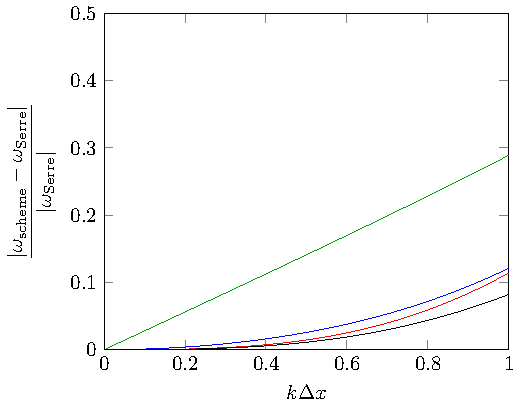
\includegraphics[width=\textwidth]{./chp5/figures/DispRelkh0p5.pdf}
		\subcaption*{\hspace{10 mm}$H = 1 $ and $k = 0.5$}
	\end{subfigure}%
	\begin{subfigure}{0.5\textwidth}
		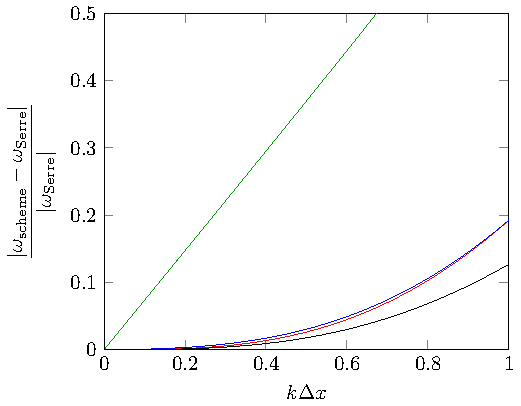
\includegraphics[width=\textwidth]{./chp5/figures/DispRelkh2p5.pdf}
		\subcaption*{\hspace{10 mm}$H = 1 $ and $k = 2.5$}
	\end{subfigure}
	\caption{Dipserion error for first-order FDVM ({\color{green!60!black} \solidrule}), second-order FDVM({\color{red} \solidrule}), second-order FEVM ({\color{blue} \solidrule})  and third-order FDVM ({\solidrule}).}
	\label{fig:DispErrMeth1}
\end{figure}

From these Figure~\ref{fig:DispErrMeth1} we can see that as expected increasing the resolution of our numerical methods decreases the dispersion error of the numerical scheme. While increasing the order of accuracy of the scheme decreases the dispersion error. 

More interesting is that the second-order FDVM performs better than the FEVM consistently across various numerical resolutions indicating that the FEVM will have a slightly larger phase error than its FDVM counterpart. Thus it appears that error in approximating $\mathcal{G}$ was more significant than the error in approximating $\mathcal{R}^{\upsilon}$ for the dispersion relation.

Our results compare well with those of \cite{Filippini-etal-2016-381} who performed a similar analysis for their numerical method applied to the linearised Serre equations with $U=0$. We have extended their results by combining the spatial and temporal contribution to the dispersion relation and performing it on a different numerical method. 

These plots only depend on the parameter $kH$. This parameter $kH$ is proportional to the shallowness parameter $\sigma$ with $2 \pi \sigma = kH $. So for $kH=2.5$ the water is no longer shallow and the Serre equations are not an appropriate model for water waves, although our results demonstrate that our numerical methods will have a small dispersion error in this case. In general, we also find that as $kH$ is increased our numerical methods perform worse generally although the dispersion relation still converges to $0$ as $\Delta x \rightarrow 0$. 


\section{Von Neumann Stability}
We will now turn our attention to demonstrating Von Neumann stability for the two finite difference methods described in this thesis $\mathcal{D}$ and $\mathcal{W}$. We shall also see that we can use some of the previous working on the dispersion relation error to demonstrate stability for our FDVM and FEVM when $U=0$. To do this as in the dispersion error analysis we will seek an equation of the form \ref{eqn:linearanalaim} relating the vector of our primitive variables at the current time to their value at the next time with an evolution matrix $\matr{E}$. If the spectral radius of the evolution matrix $\matr{E}$ is less than or equal to $1$ then our numerical scheme is stable.

To demonstrate Von Neumann stability we begin with the linearised Serre equations \eqref{eqn:LinSerre} however will no longer require $U=0$. As in the above dispersion relation analysis we will demonstrate the working in detail for one problem and then just present the results for the others. 

\subsection{Naive Second-Order Finite Difference Method $\mathcal{D}$ }
Our example will be the naive second-order finite difference method $\mathcal{D}$ \eqref{eq:Dnumdef}, which replaces all derivatives by their second-order centred finite difference approximation. For the linearised Serre equation \eqref{eqn:LinSerre} $\mathcal{D}$ is
\begin{subequations}
\begin{equation}
\eta^{n+1}_j = \eta^{n-1}_j - \Delta t \left(U \frac{- \eta^{n}_{j-1} + \eta^{n}_{j+1} }{\Delta x} + H \frac{- \upsilon^{n}_{j-1} + \upsilon^{n}_{j+1}}{\Delta x}\right),
\end{equation}
\begin{multline}
\upsilon^{n+1}_j - \frac{H^2}{3}\frac{\upsilon^{n+1}_{j-1} -2\upsilon^{n+1}_{j} +\upsilon^{n+1}_{j+1} }{\Delta x^2} 
 =  \upsilon^{n-1}_j - \frac{H^2}{3}\frac{\upsilon^{n-1}_{j-1} -2\upsilon^{n-1}_{j} +\upsilon^{n-1}_{j+1}}{\Delta x^2}   \\+  \Delta t\Bigg(- g\frac{-\eta^n_{j-1} + \eta^n_{j+1} }{\Delta x}   - U\frac{-\upsilon^n_{j-1} + \upsilon^n_{j+1} }{\Delta x}\\ + \frac{H^2}{3}\left(U \frac{-\upsilon^{n}_{j-2} +2\upsilon^{n}_{j-1} -2\upsilon^{n}_{j+1} +\upsilon^{n}_{j+2}}{\Delta x^3}  \right)\Bigg). 
\end{multline}
\label{eqn:DmethforlinSerre}
\end{subequations}


We will again assume both $\eta$ and $\upsilon$ are Fourier modes \eqref{eqn:FourierNode}. In $\mathcal{D}$ we only need to simplify 3 finite differences, which we do for a general quantity $q$ using \eqref{eqn:fourierfactor} to obtain

\begin{subequations}
	\begin{equation}
	 \frac{- q^n_{j-1} + q^n_{j+1}}{2 \Delta x} = \frac{i \sin\left(k \Delta x\right)}{\Delta x} q^n_j
	\end{equation}
	
	\begin{equation}
	\frac{q^n_{j-1} - 2q^n_j + q^n_{j+1}}{\Delta x^2} = \frac{2 \cos\left(k \Delta x\right) - 2}{\Delta x^2} q^n_j 
	\end{equation}
	\begin{equation}
	\frac{- q^n_{j-2}  + 2q^n_{j-1}  - 2q^n_{j+1} + q^n_{j+2}}{2\Delta x^3}=-4i\sin\left(k \Delta x\right)\frac{\sin^2\left(\frac{k \Delta x}{2}\right) }{\Delta x^3} q^n_j.
	\end{equation}
	\label{eqn:FDfactorlist}
\end{subequations}
Substituting in these expressions in and rearranging we get that
\begin{equation*}
\eta^{n+1}_j = \eta^{n-1}_j - \Delta t \left(U  \frac{i \sin\left(k \Delta x\right)}{\Delta x}\eta^n_j + H\frac{i \sin\left(k \Delta x\right)}{\Delta x} \upsilon^n_j \right), 
\end{equation*}
\begin{multline*}
\upsilon^{n+1}_j  =  \upsilon^{n-1}_j  -  \frac{3 \Delta x^2\Delta t}{3 \Delta x^2 -2{H^2} \left( \cos\left(k \Delta x\right) - 1 \right)}\bigg( g \frac{i \sin\left(k \Delta x\right)}{\Delta x}     \bigg) \eta^n_j\\ + U\frac{i \Delta t \sin\left(k \Delta x\right)}{\Delta x} \upsilon^n_j.  \\
\end{multline*}
 
We can rewrite this in matrix form as
\begin{equation}
\begin{bmatrix}
\eta^{n+1}_j \\
\upsilon^{n+1}_j\\
\eta^{n}_j \\
\upsilon^{n}_j
\end{bmatrix} = \matr{E}
\begin{bmatrix}
\eta^{n}_j \\
\upsilon^{n}_j\\
\eta^{n-1}_j \\
\upsilon^{n-1}_j
\end{bmatrix},
\end{equation}
where 
\begin{equation*}
\matr{E} = \begin{bmatrix}
-  \dfrac{2 i\Delta t }{\Delta x} U\sin\left(k \Delta x\right)  & -  \dfrac{2 i\Delta t}{\Delta x} H \sin\left(k \Delta x\right)  & 1 &0 \\ \\
-\dfrac{6 gi \Delta x\Delta t}{3 \Delta x^2 -2{H^2} \left( \cos\left(k \Delta x\right) - 1 \right)}{ \sin\left(k \Delta x\right)}  & -\dfrac{2i \Delta t }{\Delta x} U \sin\left(k \Delta x\right)  & 0 &1 \\
1  & 0  &0 &0 \\
0  & 1  &0 &0 
\end{bmatrix} .
\end{equation*}

This is the evolution matrix $\matr{E}$ for $\mathcal{D}$ and if its spectral radius is less than or equal to $1$ then the numerical method is stable.


\subsection{Lax-Wendroff Method $\mathcal{W}$ }
After performing the same process for the finite difference and Lax Wendroff method $\mathcal{W}$ \eqref{eq:Wnumdef} we get the following matrix equation

\begin{equation}
\begin{bmatrix}
\eta^{n+1}_j \\
\upsilon^{n+1}_j\\
\eta^n_j \\
\upsilon^n_j
\end{bmatrix}= \matr{E}  \begin{bmatrix}
\eta^{n}_j \\
\upsilon^{n}_j\\
\eta^{n-1}_j \\
\upsilon^{n-1}_j
\end{bmatrix}.
\end{equation}
where
\begin{equation}
\matr{E} = \begin{bmatrix}
{E}^{0,0} & {E}^{0,1} & 0 & - \dfrac{\Delta t}{\Delta x}H\frac{i\sin\left(k\Delta x\right)}{2} \\
{E}^{1,0} & -\dfrac{2i \Delta t }{\Delta x} U \sin\left(k \Delta x\right)&0 & 1 \\
1&0&0&0\\
0&1&0&0
\end{bmatrix}
\end{equation}
with
\begin{align*}
&{E}^{0,0} = 1 - \frac{\Delta t}{\Delta x}\left(-\dfrac{6 gi \Delta x\Delta t}{3 \Delta x^2 -2{H^2} \left( \cos\left(k \Delta x\right) - 1 \right)}{ \sin\left(k \Delta x\right)}\right)H\frac{i\sin\left(k\Delta x\right)}{2} \\ &- \frac{\Delta t}{\Delta x}U\left(\left(i\sin\left(k\Delta x\right)\right) - \frac{\Delta t}{\Delta x}U\left(\cos\left(k\Delta x\right) - 1\right)\right), \\
&{E}^{0,1} = - \frac{\Delta t}{\Delta x} \left[H\frac{i\sin\left(k\Delta x\right)}{2}\left( 1 -\dfrac{2i \Delta t }{\Delta x} U \sin\left(k \Delta x\right) \right)   -U\left(\frac{\Delta t}{\Delta x}H\left(\cos\left(k\Delta x\right) - 1\right)\right) \right],\\
& {E}^{1,0} =-\dfrac{6 gi \Delta x\Delta t}{3 \Delta x^2 -2{H^2} \left( \cos\left(k \Delta x\right) - 1 \right)}{ \sin\left(k \Delta x\right)}.
\end{align*}


\subsection{Evolution Matrices for FDVM and FEVM }
In \eqref{eqn:FullyExpandedF} we generated the evolution matrix $\matr{E}$ for the second-order FDVM when $U=0$. Applying the same process to the other numerical methods we obtain our evolution matrices for all our FDVM and FEVM so that

\begin{equation}
\begin{bmatrix}
\eta \\
\upsilon\\
\end{bmatrix}^{n+1}_j = \matr{E}  \begin{bmatrix}
\eta\\
\upsilon\
\end{bmatrix}^{n}_j .
\end{equation}
The equations for the evolution matrices are as follows, where $\matr{F}$ is the corresponding flux matrix for the numerical method.
\begin{itemize}
	\item First-order FDVM
	\[\matr{E} = \matr{I} - \Delta t \matr{F}. \]
	\item Second-order FDVM and FEVM
	\[\matr{E} = \matr{I} - \Delta t \matr{F} + \frac{1}{2} \Delta t^2 \matr{F}^2.\]
	\item Third-order FDVM
	\[\matr{E} = \matr{I} - \Delta t \matr{F} + \frac{1}{2} \Delta t^2 \matr{F}^2 - \frac{1}{6} \Delta t^3 \matr{F}^3.\]
\end{itemize}

We will now present the results of our analysis of the stability of all these methods for various $U$, $H$ and $k$ values. 

\subsection{Results}
We will demonstrate that these finite difference methods possess Von Neumann stability numerically. We do this by calculating the spectral radius of the growth matrices numerically for various fixed $H$ and $k$ values and demonstrate the behaviour of this spectral radius as $\Delta x$ changes. We use the CFL condition to determine $\Delta t$ given $\Delta x$, and in particular we again have $\Delta t =   \left( 0.5 / \left(U + \sqrt{gH}\right) \right) {\Delta x} $. We first show the results for $U = 0$ so that we  can demonstrate the stability of the FDVM and FEVM as well. We then allow various $U$ values for which we do not have the results for the FDVM and FEVM.

\subsubsection{Quiescent Fluid}
This is the situation in which we are most interested in for the purposes of ocean modelling. Most of the numerical experiments we perform later will occur in this region where the water is still with waves propagating on top. This is also the scenario in which the growth matrices for the FDVM and FEVM were calculated and thus we can only demonstrate the stability of all methods in this region. Although of course as mentioned previously the FDVM and FEVM inherit their stability from the finite volume method at their core.

The spectral radius for a range of $\Delta x$ values was plotted in Figure~\ref{fig:Stabu=0} for all numerical methods in this thesis. The representative values of $kH =0.5$ and $kH = 2.5$ were the chosen due to their use in the dispersion error analysis for the stability results plotted in Figure~\ref{fig:DispErrMeth1}. These values were representative of the results we observed for other scenarios and these values cover the range of physical scenarios we are interested in. 

Our results demonstrate that all numerical methods satisfy the stability condition for a range of $kH$ values with $U=0$ as all methods have growth matrices with spectral radius less than or equal to $1$. Indeed this is what we found generally for all these methods for all our investigated values of $hK$.

We note that both the second-order FDVM ({\color{red} \solidrule}) and FEVM ({\color{blue} \solidrule}) have very similar spectral radius values such that their plots overlap and only the curve for the FEVM ({\color{blue} \solidrule}) is visible. We also observe similar behaviour for the two second-order finite difference methods $\mathcal{D}$ ({\color{violet!80!white} \solidrule}) and $\mathcal{W}$ ({\color{orange} \solidrule}) so that only the curve for $\mathcal{W}$ ({\color{orange} \solidrule}) is visible.

We observe that the spectral radius for the second-order finite difference methods $\mathcal{D}$ and $\mathcal{W}$ are consistently $1$ when $U=0$ for various $hK$ and $
k\Delta x$ values. This can be seen in Table~\ref{tab:Averageofspectralradiusu=0}, where the average of the spectral radius for $\mathcal{D}$ and $\mathcal{W}$ over various $k \Delta x$ values is $1$ plus a number which is just the accumulation of round-off errors caused by performing this analysis numerically.
%
\begin{figure}
	\centering
	\begin{subfigure}{0.5\textwidth}
		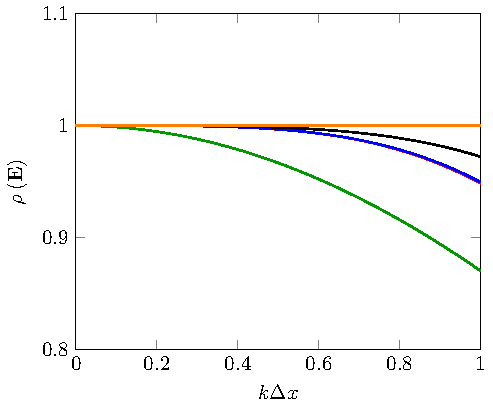
\includegraphics[width=\textwidth]{./chp5/figures/stabilityu=0kh0p5.pdf}
		\subcaption*{\hspace{10 mm}$U =0$, $H = 1 $ and $k = 0.5$}
	\end{subfigure}%
	\begin{subfigure}{0.5\textwidth}
		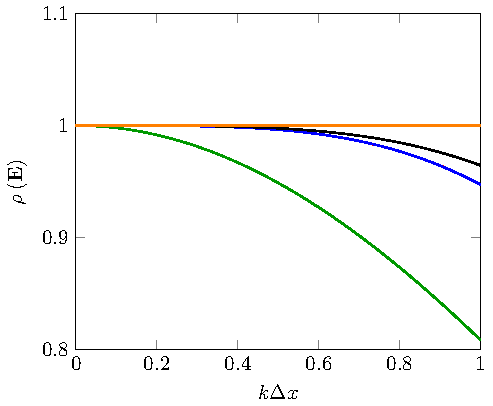
\includegraphics[width=\textwidth]{./chp5/figures/stabilityu=0kh2p5.pdf}
		\subcaption*{\hspace{10 mm}$U =0$, $H = 1 $ and $k = 2.5$}
	\end{subfigure}
	\caption{Spectral radius of growth matrix $\matr{E}$ for first-order FDVM ({\color{green!60!black} \solidrule}), second-order FDVM({\color{red} \solidrule}), second-order FEVM ({\color{blue} \solidrule}), third-order FDVM ({\solidrule}), $\mathcal{D}$ ({\color{violet!80!white} \solidrule}) and $\mathcal{W}$ ({\color{orange} \solidrule}) .}
	\label{fig:Stabu=0}
\end{figure}
%
\begin{table}
	\centering
	\begin{tabular}{l  c  c}
		\hline
		Method & $kH$& Average\\
		\hline && \\
		$\mathcal{D}$& $0.5$ & $1+ 4\times 10^{-16}$  \\
		$\mathcal{D}$& $2.5$ & $1+ 4\times 10^{-16}$  \\
		\hline \\
		$\mathcal{W}$& $0.5$ & $1+ 4\times 10^{-16}$  \\
		$\mathcal{W}$& $2.5$ & $1+ 4\times 10^{-16}$ \\
		\hline
	\end{tabular}
	\caption{Average of $\rho\left(\matr{E}\right)$ over all $\Delta x$ values for the second-order finite difference methods when $U=0$.}
	\label{tab:Averageofspectralradiusu=0}
\end{table}
\subsubsection{Non-zero Mean Flow} 
The situation of waves on still water is certainly the most common situation in ocean modelling, however there are scenarios that can arise where certain regions have a mean flow and we are interested in the waves on top, such as undular bores. Therefore we must also demonstrate stability in this case for the two finite difference methods. Since the dispersion relation analysis that derived the evolution matrix for the FDVM and FEVM assumed $U=0$ we do not demonstrate their stability here. 

We have investigated the behaviour of the spectral radius of the growth matrix for various values of $U$, $kH$ and $\Delta x$. We present the results for $U =1$ with $kH =0.5$ and $2.5$ in Figure~\ref{fig:Stabu=1}. These values were chosen because they are representative of the behaviour for both methods for most values of $U$ and $kH$, and because they match the previous values in the dispersion analysis above. 

These results demonstrate that the naive second-order method $\mathcal{D}$ is still stable even with a background mean flow, with a spectral radius that is consistently $1$. This is demonstrated in Table~\ref{tab:Averageofspectralradiusu=1} as well where the average spectral radius is $1$ plus a number that is just round-off error. This behaviour was consistent for various $U$, $kH$ and $\Delta x$ values provided the CFL condition was used to determine $\Delta t$. Therefore this method is stable as desired for a range of flow scenarios. 

Unfortunately the Lax-Wendroff finite difference method $\mathcal{W}$ is no longer stable anywhere with growth factors that are consistently larger than $1$ although it approaches stability as $\Delta x \rightarrow 0$. This is evident in Table \ref{tab:Averageofspectralradiusu=1} where the average spectral radius is larger than $1$ by significantly more than round-off error. By modifying the parameters we can increase the spectral radius as desired. However, the parameters do not follow some simple rule and their behaviour is quite complicated. Although it is the case that our largest $\Delta x$ value did correspond to our largest spectral radius. However, the interaction between the spectral radius, $hK$ and $U$ is not so obvious. Since the spectral radius was consistently larger than $1$ when $U \neq 0$ this means the Lax-Wendroff method is not stable unless $U=0$. Although the growth factors are only marginally greater than $1$ for most situations and so the instabilities may not be apparent when performing numerical experiments, as we demonstrate in Chapter []. 
\begin{figure}
	\centering
	\begin{subfigure}{0.5\textwidth}
		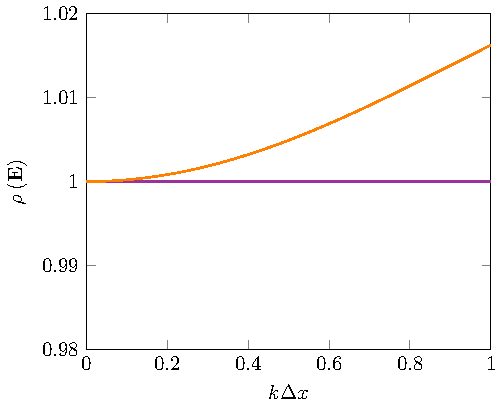
\includegraphics[width=\textwidth]{./chp5/figures/stabilityu=1kh0p5.pdf}
		\subcaption*{\hspace{10 mm}$U =1$, $H = 1 $ and $k = 0.5$}
	\end{subfigure}%
	\begin{subfigure}{0.5\textwidth}
		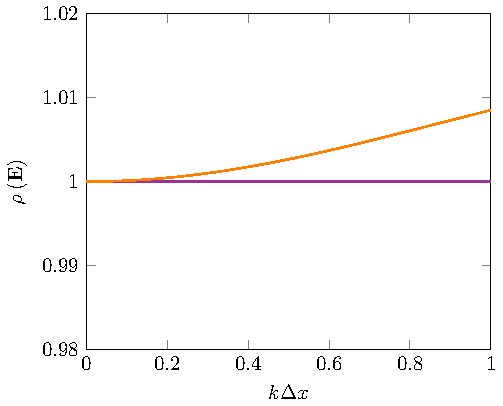
\includegraphics[width=\textwidth]{./chp5/figures/stabilityu=1kh2p5.pdf}
		\subcaption*{\hspace{10 mm}$U =1$, $H = 1 $ and $k = 2.5$}
	\end{subfigure}
	\caption{Spectral radius of growth matrix $\matr{E}$ for $\mathcal{D}$ ({\color{violet!80!white} \solidrule}) and $\mathcal{W}$ ({\color{orange} \solidrule}) .}
	\label{fig:Stabu=1}
\end{figure}


\begin{table}
	\centering
	\begin{tabular}{l  c  c}
		\hline
		Method & $kH$& Average\\
		\hline && \\
		$\mathcal{D}$ & $0.5$ & $1+ 4\times 10^{-16}$  \\
		$\mathcal{D}$ & $2.5$ & $1+ 4\times 10^{-16}$  \\
		\hline \\
		$\mathcal{W}$ & $0.5$ & $1+ 6\times 10^{-3}$  \\
		$\mathcal{W}$ & $2.5$ & $1+ 3\times 10^{-3}$   \\
		\hline
	\end{tabular}
	\caption{Average of $\rho\left(\matr{E}\right)$ over all $\Delta x$ values for the second-order finite difference methods when $U=1$.}
	\label{tab:Averageofspectralradiusu=1}
\end{table}